% Options for packages loaded elsewhere
\PassOptionsToPackage{unicode}{hyperref}
\PassOptionsToPackage{hyphens}{url}
%
\documentclass[
  letterpaper,
]{scrbook}

\usepackage{amsmath,amssymb}
\usepackage{iftex}
\ifPDFTeX
  \usepackage[T1]{fontenc}
  \usepackage[utf8]{inputenc}
  \usepackage{textcomp} % provide euro and other symbols
\else % if luatex or xetex
  \usepackage{unicode-math}
  \defaultfontfeatures{Scale=MatchLowercase}
  \defaultfontfeatures[\rmfamily]{Ligatures=TeX,Scale=1}
\fi
\usepackage{lmodern}
\ifPDFTeX\else  
    % xetex/luatex font selection
\fi
% Use upquote if available, for straight quotes in verbatim environments
\IfFileExists{upquote.sty}{\usepackage{upquote}}{}
\IfFileExists{microtype.sty}{% use microtype if available
  \usepackage[]{microtype}
  \UseMicrotypeSet[protrusion]{basicmath} % disable protrusion for tt fonts
}{}
\makeatletter
\@ifundefined{KOMAClassName}{% if non-KOMA class
  \IfFileExists{parskip.sty}{%
    \usepackage{parskip}
  }{% else
    \setlength{\parindent}{0pt}
    \setlength{\parskip}{6pt plus 2pt minus 1pt}}
}{% if KOMA class
  \KOMAoptions{parskip=half}}
\makeatother
\usepackage{xcolor}
\usepackage[margin=2.5cm]{geometry}
\setlength{\emergencystretch}{3em} % prevent overfull lines
\setcounter{secnumdepth}{5}
% Make \paragraph and \subparagraph free-standing
\ifx\paragraph\undefined\else
  \let\oldparagraph\paragraph
  \renewcommand{\paragraph}[1]{\oldparagraph{#1}\mbox{}}
\fi
\ifx\subparagraph\undefined\else
  \let\oldsubparagraph\subparagraph
  \renewcommand{\subparagraph}[1]{\oldsubparagraph{#1}\mbox{}}
\fi


\providecommand{\tightlist}{%
  \setlength{\itemsep}{0pt}\setlength{\parskip}{0pt}}\usepackage{longtable,booktabs,array}
\usepackage{calc} % for calculating minipage widths
% Correct order of tables after \paragraph or \subparagraph
\usepackage{etoolbox}
\makeatletter
\patchcmd\longtable{\par}{\if@noskipsec\mbox{}\fi\par}{}{}
\makeatother
% Allow footnotes in longtable head/foot
\IfFileExists{footnotehyper.sty}{\usepackage{footnotehyper}}{\usepackage{footnote}}
\makesavenoteenv{longtable}
\usepackage{graphicx}
\makeatletter
\def\maxwidth{\ifdim\Gin@nat@width>\linewidth\linewidth\else\Gin@nat@width\fi}
\def\maxheight{\ifdim\Gin@nat@height>\textheight\textheight\else\Gin@nat@height\fi}
\makeatother
% Scale images if necessary, so that they will not overflow the page
% margins by default, and it is still possible to overwrite the defaults
% using explicit options in \includegraphics[width, height, ...]{}
\setkeys{Gin}{width=\maxwidth,height=\maxheight,keepaspectratio}
% Set default figure placement to htbp
\makeatletter
\def\fps@figure{htbp}
\makeatother

\makeatletter
\@ifpackageloaded{tcolorbox}{}{\usepackage[skins,breakable]{tcolorbox}}
\@ifpackageloaded{fontawesome5}{}{\usepackage{fontawesome5}}
\definecolor{quarto-callout-color}{HTML}{909090}
\definecolor{quarto-callout-note-color}{HTML}{0758E5}
\definecolor{quarto-callout-important-color}{HTML}{CC1914}
\definecolor{quarto-callout-warning-color}{HTML}{EB9113}
\definecolor{quarto-callout-tip-color}{HTML}{00A047}
\definecolor{quarto-callout-caution-color}{HTML}{FC5300}
\definecolor{quarto-callout-color-frame}{HTML}{acacac}
\definecolor{quarto-callout-note-color-frame}{HTML}{4582ec}
\definecolor{quarto-callout-important-color-frame}{HTML}{d9534f}
\definecolor{quarto-callout-warning-color-frame}{HTML}{f0ad4e}
\definecolor{quarto-callout-tip-color-frame}{HTML}{02b875}
\definecolor{quarto-callout-caution-color-frame}{HTML}{fd7e14}
\makeatother
\makeatletter
\makeatother
\makeatletter
\@ifpackageloaded{bookmark}{}{\usepackage{bookmark}}
\makeatother
\makeatletter
\@ifpackageloaded{caption}{}{\usepackage{caption}}
\AtBeginDocument{%
\ifdefined\contentsname
  \renewcommand*\contentsname{Table of contents}
\else
  \newcommand\contentsname{Table of contents}
\fi
\ifdefined\listfigurename
  \renewcommand*\listfigurename{List of Figures}
\else
  \newcommand\listfigurename{List of Figures}
\fi
\ifdefined\listtablename
  \renewcommand*\listtablename{List of Tables}
\else
  \newcommand\listtablename{List of Tables}
\fi
\ifdefined\figurename
  \renewcommand*\figurename{Figure}
\else
  \newcommand\figurename{Figure}
\fi
\ifdefined\tablename
  \renewcommand*\tablename{Table}
\else
  \newcommand\tablename{Table}
\fi
}
\@ifpackageloaded{float}{}{\usepackage{float}}
\floatstyle{ruled}
\@ifundefined{c@chapter}{\newfloat{codelisting}{h}{lop}}{\newfloat{codelisting}{h}{lop}[chapter]}
\floatname{codelisting}{Listing}
\newcommand*\listoflistings{\listof{codelisting}{List of Listings}}
\makeatother
\makeatletter
\@ifpackageloaded{caption}{}{\usepackage{caption}}
\@ifpackageloaded{subcaption}{}{\usepackage{subcaption}}
\makeatother
\makeatletter
\@ifpackageloaded{tcolorbox}{}{\usepackage[skins,breakable]{tcolorbox}}
\makeatother
\makeatletter
\@ifundefined{shadecolor}{\definecolor{shadecolor}{rgb}{.97, .97, .97}}
\makeatother
\makeatletter
\makeatother
\makeatletter
\makeatother
\ifLuaTeX
  \usepackage{selnolig}  % disable illegal ligatures
\fi
\IfFileExists{bookmark.sty}{\usepackage{bookmark}}{\usepackage{hyperref}}
\IfFileExists{xurl.sty}{\usepackage{xurl}}{} % add URL line breaks if available
\urlstyle{same} % disable monospaced font for URLs
\hypersetup{
  pdftitle={COURSE TITLE},
  pdfauthor={YOUR NAME},
  hidelinks,
  pdfcreator={LaTeX via pandoc}}

\title{COURSE TITLE}
\author{YOUR NAME}
\date{2026-07-12}

\begin{document}
\frontmatter
\maketitle
\ifdefined\Shaded\renewenvironment{Shaded}{\begin{tcolorbox}[boxrule=0pt, sharp corners, enhanced, interior hidden, borderline west={3pt}{0pt}{shadecolor}, breakable, frame hidden]}{\end{tcolorbox}}\fi

\renewcommand*\contentsname{Table of contents}
{
\setcounter{tocdepth}{2}
\tableofcontents
}
\mainmatter
\bookmarksetup{startatroot}

\hypertarget{bienvenue}{%
\chapter*{Bienvenue}\label{bienvenue}}
\addcontentsline{toc}{chapter}{Bienvenue}

\markboth{Bienvenue}{Bienvenue}

Landing page for the book version of this course. Short description of
the course, how it's organized, and a link to the slide decks (which
live outside the book navigation, under \texttt{decks/}).

\bookmarksetup{startatroot}

\hypertarget{introduction-uxe0-la-linguistique-diachronique}{%
\chapter{Introduction à la linguistique
diachronique}\label{introduction-uxe0-la-linguistique-diachronique}}

\hypertarget{linguistique-vs-grammaire}{%
\section{Linguistique vs grammaire}\label{linguistique-vs-grammaire}}

\hypertarget{le-lemme-linguistique-dans-le-tlfi}{%
\subsection{\texorpdfstring{Le lemme \emph{linguistique} dans le
TLFi}{Le lemme linguistique dans le TLFi}}\label{le-lemme-linguistique-dans-le-tlfi}}

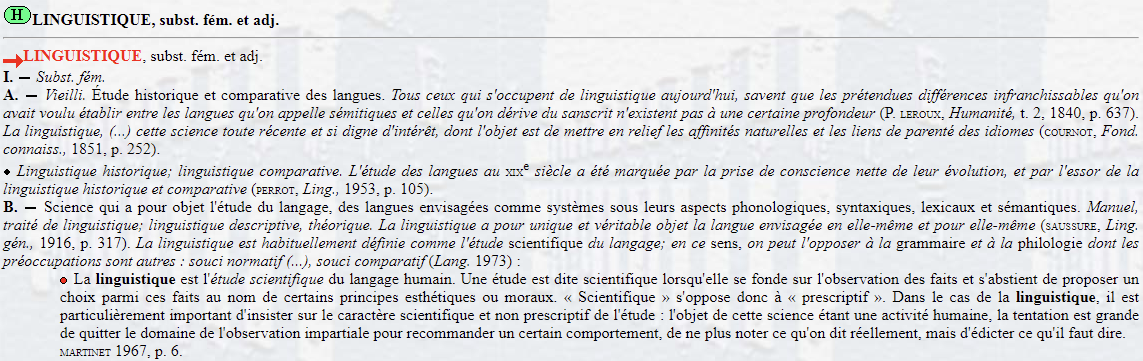
\includegraphics{chapters/images/clipboard-3754285985.png}

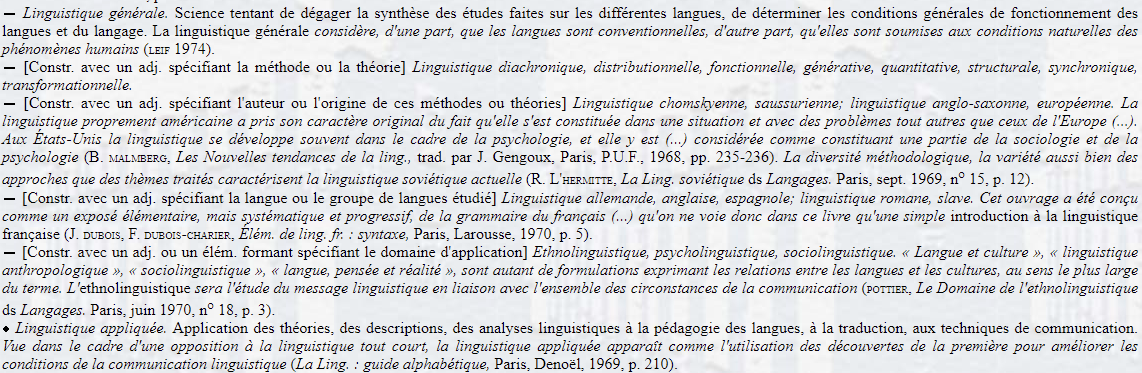
\includegraphics{chapters/images/clipboard-1683819146.png}

\hypertarget{le-lemme-grammaire-dans-le-tlfi}{%
\subsection{\texorpdfstring{Le lemme \emph{grammaire} dans le
TLFi}{Le lemme grammaire dans le TLFi}}\label{le-lemme-grammaire-dans-le-tlfi}}

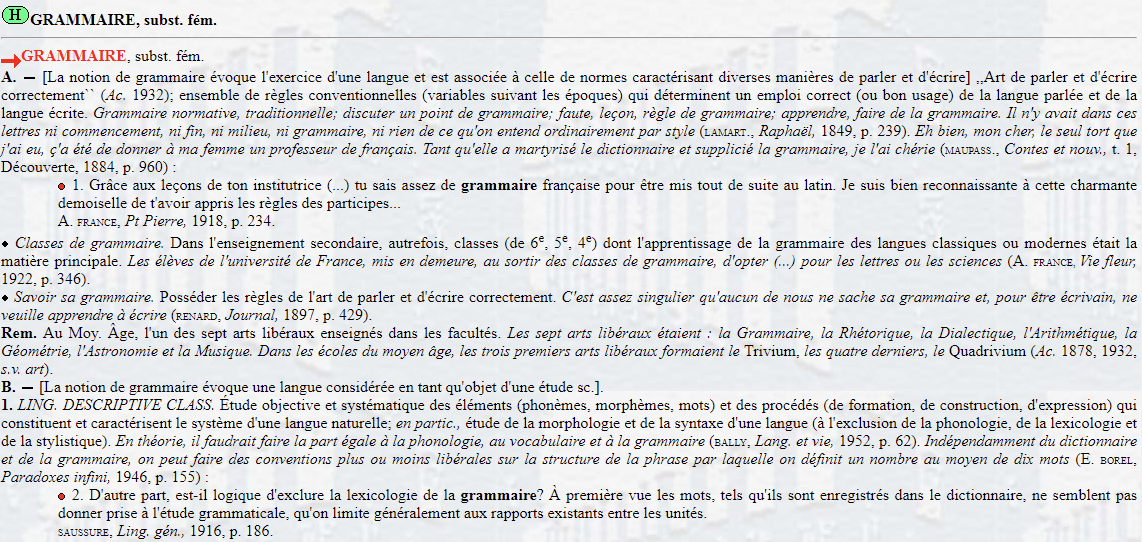
\includegraphics{chapters/images/clipboard-658805517.png}

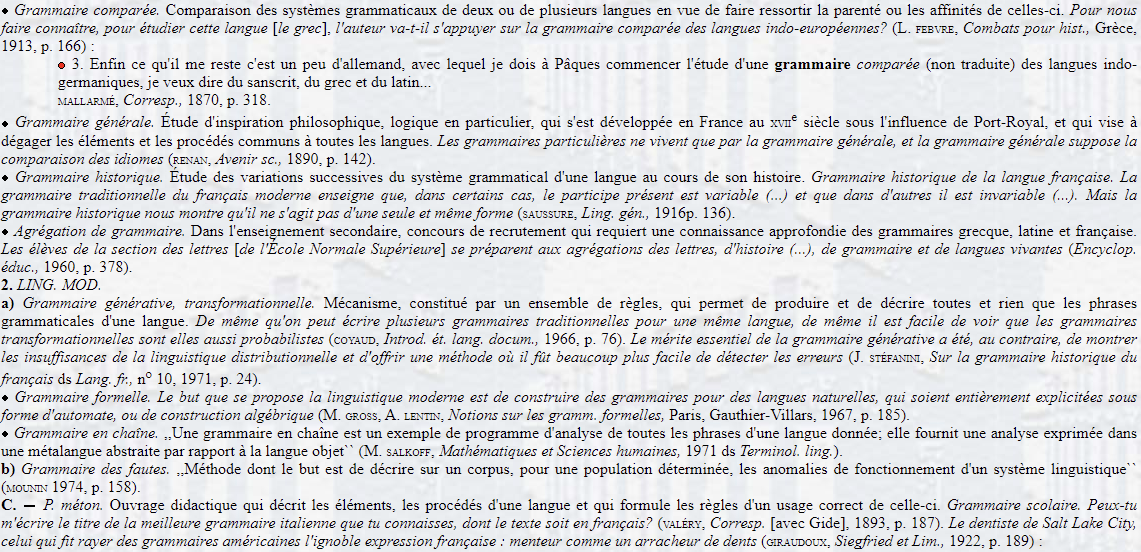
\includegraphics{chapters/images/clipboard-2109517839.png}

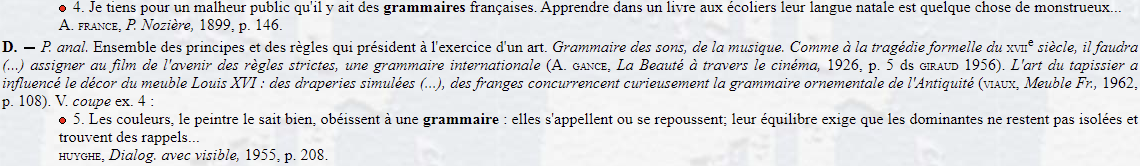
\includegraphics{chapters/images/clipboard-1197071049.png}

\hypertarget{linguistique-vs-grammaire-deux-disciplines-scientifiques-ayant-pour-objet-duxe9tude-la-langue-sous-diffuxe9rents-aspects}{%
\subsection{Linguistique vs grammaire : deux disciplines scientifiques
ayant pour objet d'étude la langue « sous différents aspects
»}\label{linguistique-vs-grammaire-deux-disciplines-scientifiques-ayant-pour-objet-duxe9tude-la-langue-sous-diffuxe9rents-aspects}}

\hypertarget{quatre-diffuxe9rences-fondamentales}{%
\subsubsection{Quatre différences fondamentales
:}\label{quatre-diffuxe9rences-fondamentales}}

\begin{itemize}
\item
  Objet d'étude
\item
  Objectif poursuivi
\item
  Organisation de la description
\item
  Terminologie utilisée
\end{itemize}

Un regard plus profond sur ces critères permet non seulement d'opposer
grammaire à linguistique, mais aussi d'introduire les concepts de
grammaire émergente et de changement linguistique.

\hypertarget{objet-duxe9tude}{%
\section{Objet d'étude}\label{objet-duxe9tude}}

Toute variété linguistique se définit par un faisceau unique de
variables diasystémiques :

\hypertarget{les-dimensions-de-la-variation}{%
\subsection{Les dimensions de la
variation}\label{les-dimensions-de-la-variation}}

\hypertarget{variation-diachronique}{%
\subsubsection{Variation diachronique}\label{variation-diachronique}}

Exemple : Les Serments de Strasbourg (842) vs français moderne

\begin{longtable}[]{@{}ll@{}}
\toprule\noalign{}
Très ancien français & Français moderne \\
\midrule\noalign{}
\endhead
\bottomrule\noalign{}
\endlastfoot
\emph{Pro Deo amur\ldots{}} & \emph{Pour l'amour de Dieu\ldots{}} \\
\end{longtable}

Exemple : négation ancien français vs contemporain

\begin{enumerate}
\def\labelenumi{\arabic{enumi}.}
\item
  \emph{Jeo ne mange.}
\item
  \emph{Je ne mange pas.}
\end{enumerate}

\hypertarget{variation-diatopique}{%
\subsubsection{Variation diatopique}\label{variation-diatopique}}

\begin{figure}

{\centering 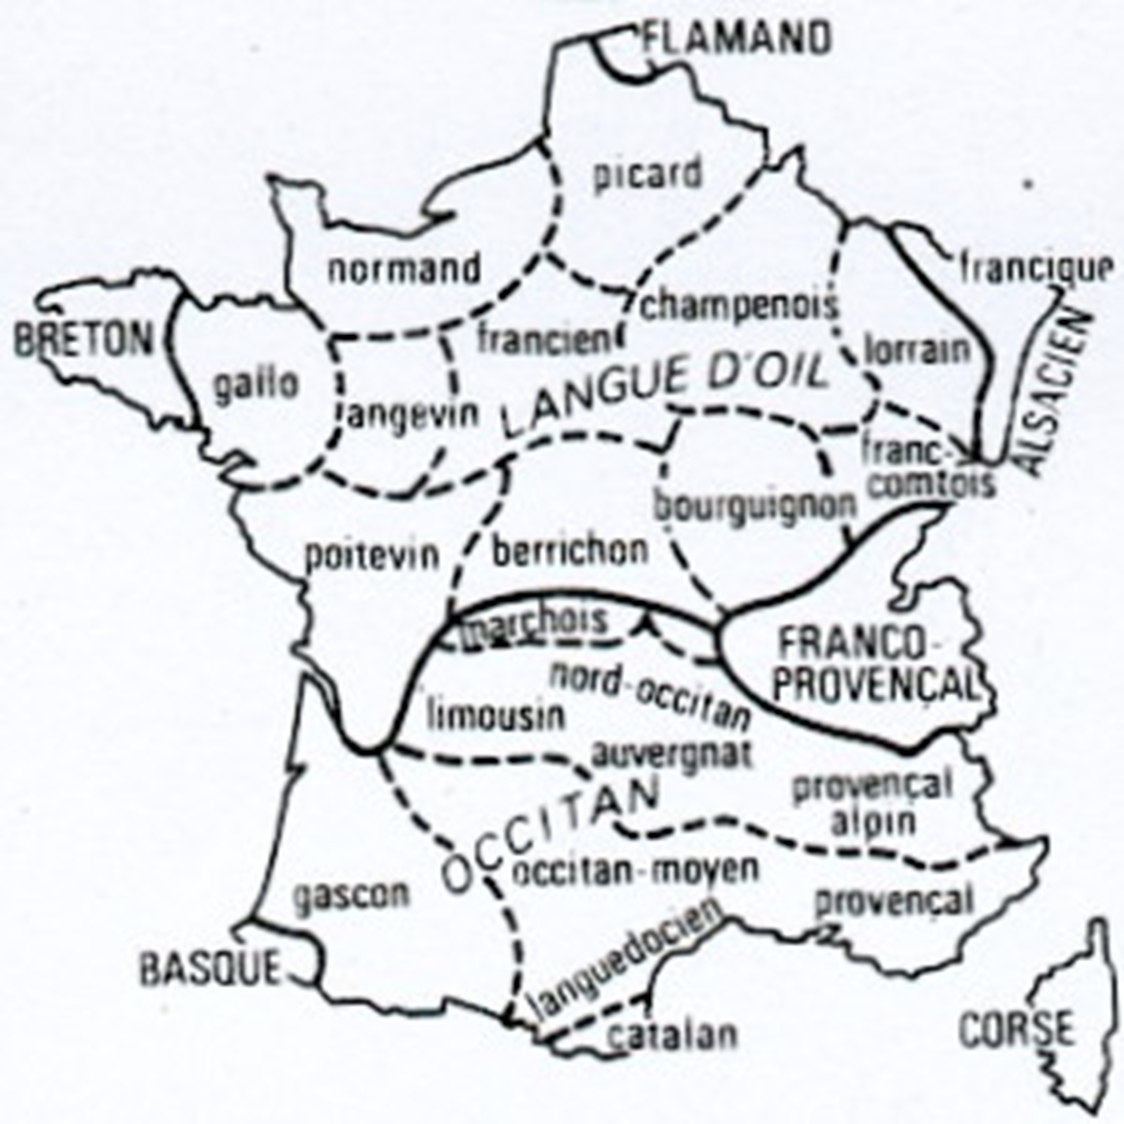
\includegraphics{chapters/images/clipboard-1931647397.png}

}

\caption{La variation dialectale en France}

\end{figure}

Variation phonétique Paris vs Midi

\begin{longtable}[]{@{}ll@{}}
\toprule\noalign{}
Paris & Midi \\
\midrule\noalign{}
\endhead
\bottomrule\noalign{}
\endlastfoot
le lait → {[}lǝlɜ{]} & {[}lǝle{]} \\
aimerais / aimerai → {[}emʁɜ{]} / {[}emʁe{]} & {[}eməre{]} \\
\end{longtable}

Genre des emprunts anglais : France vs Canada

\begin{longtable}[]{@{}lll@{}}
\toprule\noalign{}
Anglais & France & Canada \\
\midrule\noalign{}
\endhead
\bottomrule\noalign{}
\endlastfoot
the job & le job & la job \\
the gang & le gang & la gang \\
\end{longtable}

Chiffres 70 et 90 : France vs Belgique/Suisse

\begin{longtable}[]{@{}ll@{}}
\toprule\noalign{}
France & Belgique/Suisse \\
\midrule\noalign{}
\endhead
\bottomrule\noalign{}
\endlastfoot
soixante-dix & septante \\
quatre-vingt-dix & nonante \\
\end{longtable}

\hypertarget{variation-diastratique}{%
\subsubsection{Variation diastratique}\label{variation-diastratique}}

Langue des jeunes :

\begin{itemize}
\item
  \emph{staïve}, \emph{balec}
\item
  \emph{stremon}, \emph{meuf}, \emph{tromé}
\end{itemize}

\hypertarget{variation-diaphasique}{%
\subsubsection{Variation diaphasique}\label{variation-diaphasique}}

Registre soutenu vs familier

\begin{longtable}[]{@{}ll@{}}
\toprule\noalign{}
Soutenu & Familier \\
\midrule\noalign{}
\endhead
\bottomrule\noalign{}
\endlastfoot
Bonjour ! & Salut ! \\
Pas de problème. & Pas d'problème. \\
Je ne sais pas\ldots{} & Je sais pas\ldots{} \\
\end{longtable}

\hypertarget{variation-diamuxe9sique}{%
\subsubsection{Variation diamésique}\label{variation-diamuxe9sique}}

Écrit vs oral

\begin{longtable}[]{@{}ll@{}}
\toprule\noalign{}
Écrit & Oral \\
\midrule\noalign{}
\endhead
\bottomrule\noalign{}
\endlastfoot
Bonjour ! & Salut ! \\
Il y a plusieurs façons\ldots{} & Y'a plusieurs façons\ldots{} \\
\end{longtable}

\hypertarget{paramuxe8tres-diasystuxe9miques-scalaires}{%
\subsubsection{Paramètres diasystémiques =
scalaires}\label{paramuxe8tres-diasystuxe9miques-scalaires}}

Exemple : continuum diachronique latin → ancien français → moderne

\emph{(tableau conservé)}

\begin{figure}

{\centering 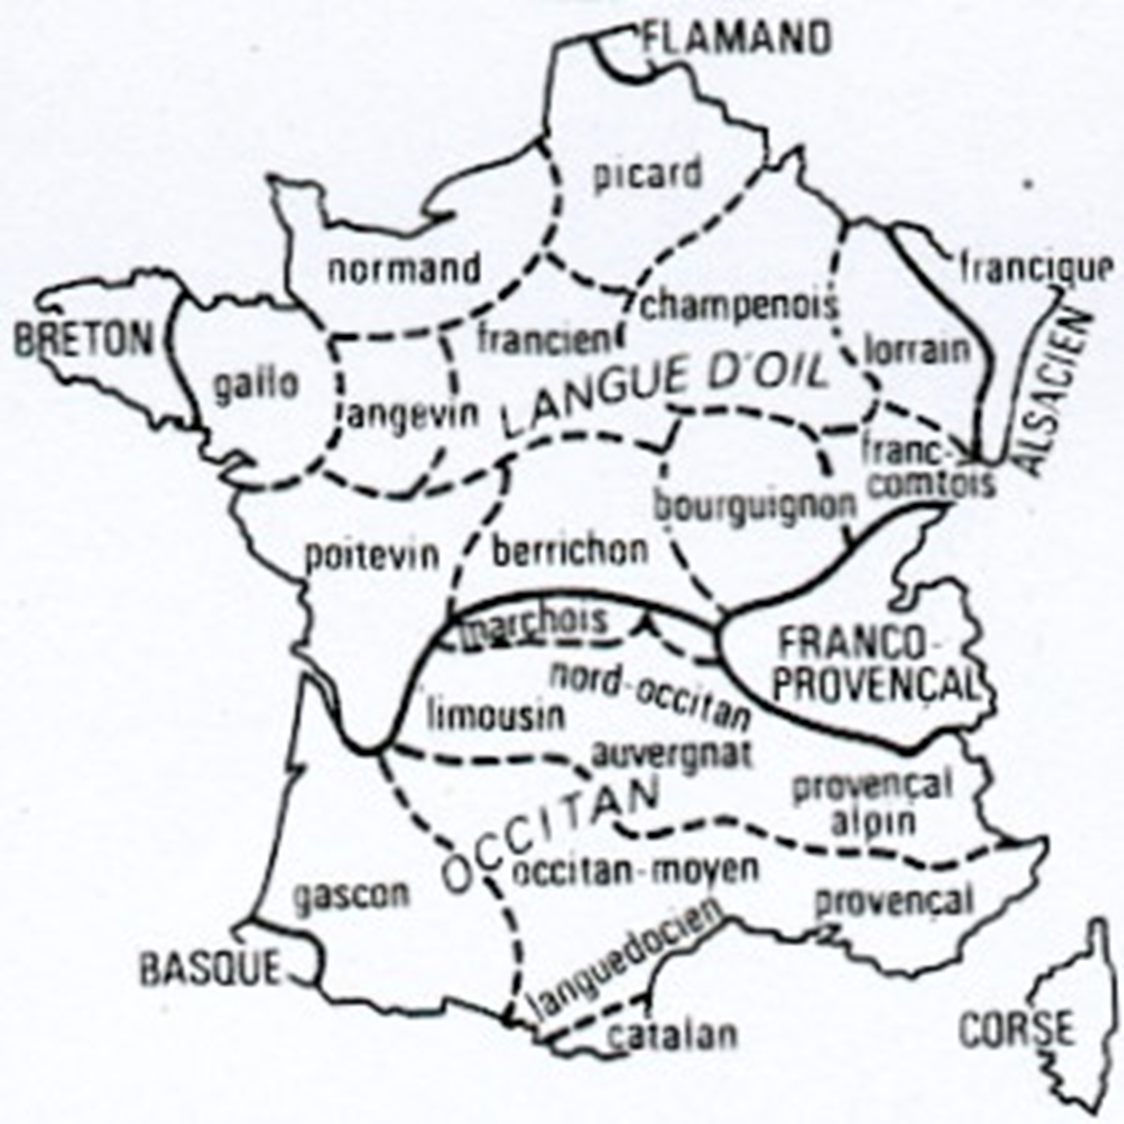
\includegraphics{chapters/images/clipboard-3434876068.png}

}

\caption{Continuum langues d'oc / langues d'oïl}

\end{figure}

\hypertarget{et-alors-quelles-variuxe9tuxe9s-uxe9tudie-t-on}{%
\section{Et alors, quelles variétés
étudie-t-on?}\label{et-alors-quelles-variuxe9tuxe9s-uxe9tudie-t-on}}

\begin{itemize}
\tightlist
\item
  Linguistes : toutes les variétés
\end{itemize}

\begin{itemize}
\tightlist
\item
  Grammairiens : langue écrite des « bons écrivains »
\end{itemize}

\hypertarget{consuxe9quences-pour-la-grammaire}{%
\subsubsection{Conséquences pour la
grammaire}\label{consuxe9quences-pour-la-grammaire}}

Les grammairiens décrivent un bon usage basé sur une variété écrite,
souvent en décalage avec l'usage réel.

\hypertarget{duxe9viations-et-changement-linguistique}{%
\subsubsection{Déviations et changement
linguistique}\label{duxe9viations-et-changement-linguistique}}

\begin{quote}
« La faute d'aujourd'hui est la norme de demain. » --- A. Rey
\end{quote}

\begin{itemize}
\item
  Les déviations = innovations
\item
  Le changement = conventionnalisation de ces innovations
\end{itemize}

\hypertarget{objectif-poursuivi}{%
\section{Objectif poursuivi}\label{objectif-poursuivi}}

\hypertarget{deux-objectifs}{%
\subsection{Deux objectifs :}\label{deux-objectifs}}

\begin{itemize}
\item
  Grammairien : prescriptif / normatif
\item
  Linguiste : descriptif / explicatif
\end{itemize}

\hypertarget{attitude-face-aux-duxe9viations}{%
\subsection{Attitude face aux déviations
:}\label{attitude-face-aux-duxe9viations}}

\begin{itemize}
\item
  Grammairien → fautes
\item
  Linguiste → alternatives à décrire
\end{itemize}

\hypertarget{exemple-duxe9tailluxe9-la-nuxe9gation}{%
\section{Exemple détaillé : la
négation}\label{exemple-duxe9tailluxe9-la-nuxe9gation}}

Évolution de \emph{pas} et \emph{mie} du latin au français moderne
(tableaux conservés).

\hypertarget{exemple-le-genre-de-espuxe8ce}{%
\section{\texorpdfstring{Exemple : le genre de
\emph{espèce}}{Exemple : le genre de espèce}}\label{exemple-le-genre-de-espuxe8ce}}

\hypertarget{questions}{%
\subsection{Questions :}\label{questions}}

\begin{enumerate}
\def\labelenumi{\arabic{enumi}.}
\item
  Quel est son genre ?
\item
  Quel est son emploi réel ?
\item
  Attitude grammairien vs linguiste
\item
  Explication de l'emploi déviant
\end{enumerate}

\hypertarget{ruxe9fuxe9rence-grammaticale}{%
\subsection{Référence grammaticale}\label{ruxe9fuxe9rence-grammaticale}}

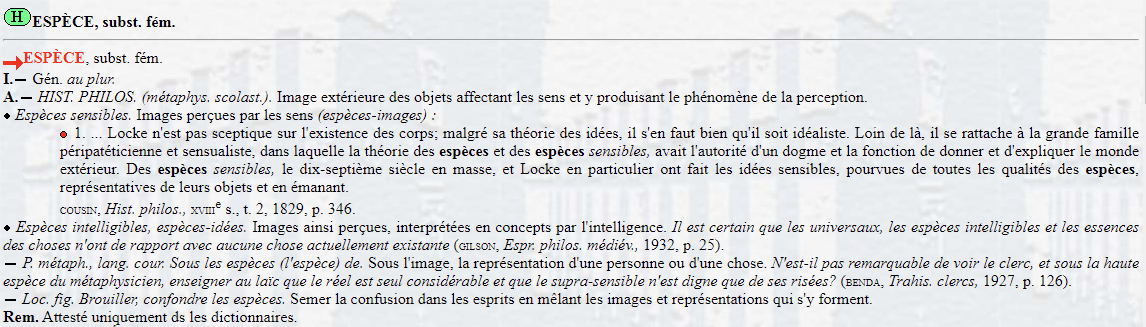
\includegraphics{chapters/images/clipboard-2485027561.png}

\begin{center}\rule{0.5\linewidth}{0.5pt}\end{center}

\hypertarget{les-donnuxe9es-ruxe9elles}{%
\subsection{Les données réelles}\label{les-donnuxe9es-ruxe9elles}}

Observez les exemples ci-dessous et dégagez-en les règles qui régissent
le genre du mot \emph{espèce}.

\begin{enumerate}
\def\labelenumi{\arabic{enumi}.}
\item
  Une espèce de con.
\item
  Une espèce de crapule.
\item
  Un espèce de moteur.
\item
  Une espèce de voiture.
\item
  Un espèce d'individu.
\item
  Une espèce de fleur.
\item
  Un espèce de problème.
\end{enumerate}

\begin{center}\rule{0.5\linewidth}{0.5pt}\end{center}

\hypertarget{la-ruxe9ponse-du-grammairien}{%
\subsection{La réponse du
grammairien}\label{la-ruxe9ponse-du-grammairien}}

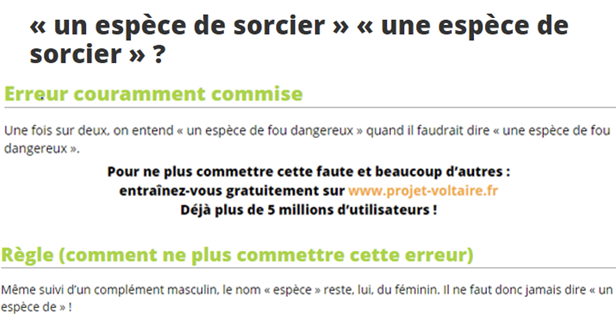
\includegraphics{chapters/images/clipboard-1591005596.png}

\begin{center}\rule{0.5\linewidth}{0.5pt}\end{center}

\hypertarget{la-ruxe9ponse-du-linguiste}{%
\subsection{La réponse du linguiste}\label{la-ruxe9ponse-du-linguiste}}

\hypertarget{e-uxe9tape-description-du-phuxe9nomuxe8ne}{%
\subsubsection{1e étape : description du
phénomène}\label{e-uxe9tape-description-du-phuxe9nomuxe8ne}}

\begin{enumerate}
\def\labelenumi{\arabic{enumi}.}
\item
  Malgré son genre inhérent qui est le féminin, le genre du mot espèce
  tend à varier
\item
  Le genre du mot espèce ne varie que dans la construction {[}DET espèce
  de N{]} :

  \begin{enumerate}
  \def\labelenumii{\arabic{enumii}.}
  \item
    Il ne connaît pas cette espèce.
  \item
    *Il ne connaît pas cet espèce.
  \end{enumerate}
\item
  Le genre du mot espèce peut être féminin peu importe le genre du N qui
  suit la préposition de :

  \begin{enumerate}
  \def\labelenumii{\arabic{enumii}.}
  \item
    Une espèce de voiture.
  \item
    Une espèce de problème.
  \end{enumerate}
\item
  Le genre du mot espèce peut être masculin seulement si le genre du N
  qui suit la préposition de est masculin :

  \begin{enumerate}
  \def\labelenumii{\arabic{enumii}.}
  \item
    Un espèce de problème.
  \item
    *Un espèce de voiture.
  \end{enumerate}
\end{enumerate}

\begin{center}\rule{0.5\linewidth}{0.5pt}\end{center}

\hypertarget{e-uxe9tape-explication-du-phuxe9nomuxe8ne}{%
\subsubsection{2e étape : explication du
phénomène}\label{e-uxe9tape-explication-du-phuxe9nomuxe8ne}}

\begin{center}\rule{0.5\linewidth}{0.5pt}\end{center}

\hypertarget{analyse}{%
\subsection{Analyse :}\label{analyse}}

\begin{itemize}
\item
  \emph{espèce} = féminin inhérent
\item
  Variation uniquement dans {[}DET espèce de N{]}
\item
  Masculin possible seulement si N est masculin
\item
  Réanalyse : \emph{une espèce de N} → déterminant complexe
\item
  Évolution en cours : coexistence des deux formes
\end{itemize}

\hypertarget{linguistique-synchronique-vs-diachronique-vs-historique}{%
\section{Linguistique synchronique vs diachronique vs
historique}\label{linguistique-synchronique-vs-diachronique-vs-historique}}

\hypertarget{synchronie}{%
\subsection{Synchronie}\label{synchronie}}

\begin{tcolorbox}[enhanced jigsaw, colframe=quarto-callout-note-color-frame, breakable, opacitybacktitle=0.6, arc=.35mm, toprule=.15mm, colbacktitle=quarto-callout-note-color!10!white, colback=white, opacityback=0, bottomtitle=1mm, toptitle=1mm, titlerule=0mm, bottomrule=.15mm, left=2mm, coltitle=black, title=\textcolor{quarto-callout-note-color}{\faInfo}\hspace{0.5em}{Note}, rightrule=.15mm, leftrule=.75mm]

Synchronie \textgreater{} gr. σύν `avec' (lat. syn) + χρόνος `temps'
(lat. chronos)

\end{tcolorbox}

• La position de la femme en Europe au Moyen Age

• L'économie de la France au 21e s.

• L'expression de la négation en ancien français

• \ldots{}

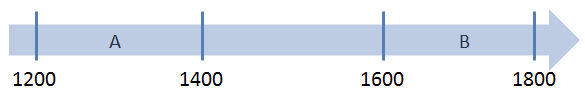
\includegraphics{chapters/images/clipboard-1877567029.png}

🚨 Synchronie du passé

\hypertarget{diachronie}{%
\subsection{Diachronie}\label{diachronie}}

\begin{tcolorbox}[enhanced jigsaw, colframe=quarto-callout-note-color-frame, breakable, opacitybacktitle=0.6, arc=.35mm, toprule=.15mm, colbacktitle=quarto-callout-note-color!10!white, colback=white, opacityback=0, bottomtitle=1mm, toptitle=1mm, titlerule=0mm, bottomrule=.15mm, left=2mm, coltitle=black, title=\textcolor{quarto-callout-note-color}{\faInfo}\hspace{0.5em}{Note}, rightrule=.15mm, leftrule=.75mm]

Diachronie \textgreater{} διά `à travers' (lat. dia) + χρόνος `temps'
(lat. chronos)

\end{tcolorbox}

• La position de la femme en Europe du Moyen Age au 20ième s.

• L'économie de la France du 19ième au 21ième s.

• L'expression de la négation de l'ancien français au français classique

• \ldots{}

\begin{center}\rule{0.5\linewidth}{0.5pt}\end{center}

\includegraphics{chapters/images/Metal_voice.mp4}

\includegraphics{chapters/images/Vocal Fry.mp4}Î

\begin{center}\rule{0.5\linewidth}{0.5pt}\end{center}

\begin{enumerate}
\def\labelenumi{\arabic{enumi}.}
\tightlist
\item
  Genève 🇨🇭
\item
  Études de linguistique historique à l'Université de Leipzig, doctorat
  en 1879
\item
  Mémoire sur le système primitif des voyelles indo-européennes (1877)
\item
  1881 : Maître de conférences à Paris
\item
  1892 : Université de Genève
\item
  1906--1913 : Chaire de linguistique générale
\end{enumerate}

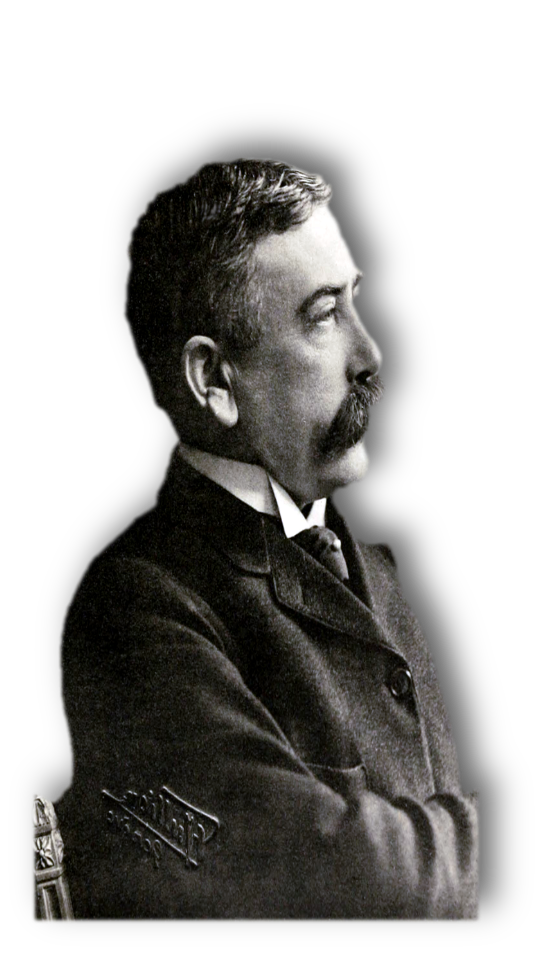
\includegraphics[width=1\textwidth,height=\textheight]{chapters/images/clipboard-1008386988.png}


\includegraphics{chapters/images/clipboard-562782746.png}

\hypertarget{historique}{%
\subsection{Historique}\label{historique}}

Histoire externe : substrats, superstrats, adstrats.

\hypertarget{intuxe9ruxeat-de-la-linguistique-diachronique}{%
\section{Intérêt de la linguistique
diachronique}\label{intuxe9ruxeat-de-la-linguistique-diachronique}}

\begin{itemize}
\item
  Comprendre le fonctionnement de la langue
\item
  Typologie → prédictions
\item
  Cognition humaine
\item
  Comprendre des faits synchroniques
\end{itemize}

\hypertarget{perception-du-changement-linguistique}{%
\section{Perception du changement
linguistique}\label{perception-du-changement-linguistique}}

\hypertarget{passuxe9}{%
\subsection{Passé :}\label{passuxe9}}

\begin{itemize}
\item
  Idéalisation du latin, du grec
\item
  Vision décadente du changement
\end{itemize}

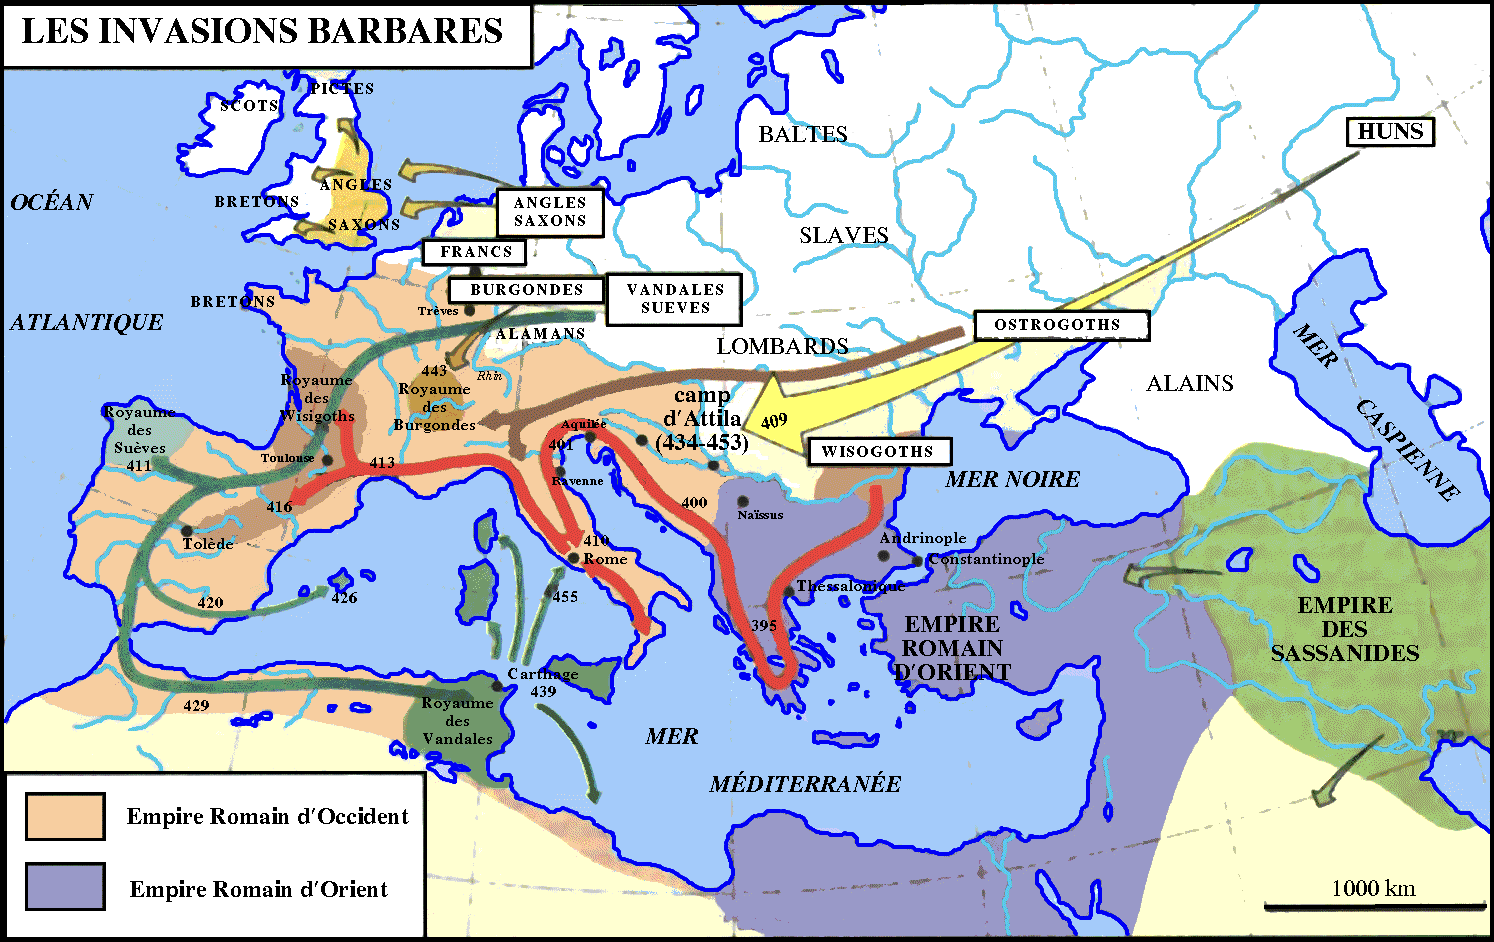
\includegraphics{chapters/images/clipboard-2388570064.png}

\hypertarget{aujourdhui}{%
\subsection{Aujourd'hui :}\label{aujourdhui}}

\begin{itemize}
\item
  Neutralité pour le passé
\item
  Normativité pour le présent
\end{itemize}

\hypertarget{changement-signe-de-vie}{%
\subsection{Changement = signe de vie}\label{changement-signe-de-vie}}

\hypertarget{raisons-de-laccuxe9luxe9ration}{%
\subsection{Raisons de l'accélération
:}\label{raisons-de-laccuxe9luxe9ration}}

\begin{itemize}
\item
  Mondialisation
\item
  Internet, réseaux sociaux
\end{itemize}

\hypertarget{section}{%
\section{}\label{section}}

\hypertarget{perception-du-changement-linguistique-1}{%
\section{Perception du changement
linguistique}\label{perception-du-changement-linguistique-1}}

\hypertarget{dans-le-passuxe9-surtout-au-19iuxe8me-s.}{%
\subsection{Dans le passé (surtout au 19ième s.)
:}\label{dans-le-passuxe9-surtout-au-19iuxe8me-s.}}

\begin{quote}
« Plus on remonte dans le temps, plus la forme du langage est belle et
parfaite. Plus on s'approche du présent, plus il est pénible de trouver
au langage, en décadence, de la force et de la flexibilité. » (Jacob \&
Guillaume Grimm)
\end{quote}

\begin{quote}
« Les langues à flexion qui sont tombées aujourd'hui en ruines ne
pourront jamais de nouveau se relever à leur hauteur primitive. »
(August Schleicher)
\end{quote}

\hypertarget{perception-traditionnelle}{%
\subsection{Perception traditionnelle
:}\label{perception-traditionnelle}}

\begin{itemize}
\item
  Primauté des langues classiques (grec ancien, latin, sanscrit, etc.)
\item
  La disparition de ces langues est déplorable : dégénération, décadence
\item
  Langues flexionnelles \textgreater{} langues non flexionnelles
\item
  Idéalisation des systèmes linguistiques du passé, mépris des systèmes
  linguistiques contemporains et désespoir des systèmes linguistiques
  futurs
\end{itemize}

\begin{center}\rule{0.5\linewidth}{0.5pt}\end{center}

Comme si en biologie\ldots{}

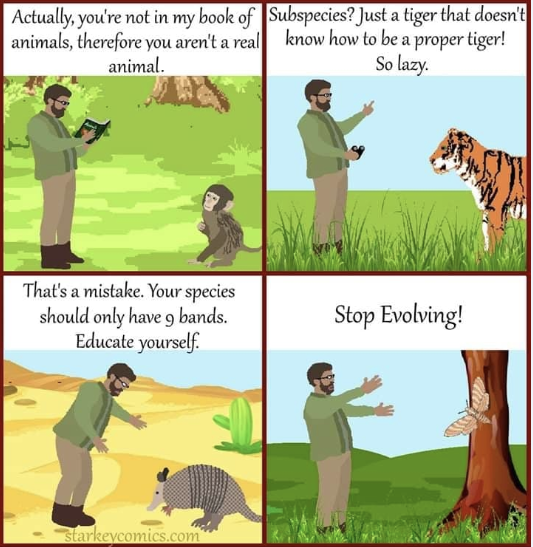
\includegraphics{chapters/images/clipboard-1698630812.png}

\hypertarget{difficultuxe9s-muxe9thodologiques-propres-uxe0-la-linguistique-diachronique}{%
\section{Difficultés méthodologiques propres à la linguistique
diachronique}\label{difficultuxe9s-muxe9thodologiques-propres-uxe0-la-linguistique-diachronique}}

Besoin d'une base empirique : un corpus solide et représentatif de
textes authentiques couvrant des périodes plus ou moins étendues

dépendance de la transmission textuelle

\hypertarget{probluxe8mes}{%
\subsection{Problèmes :}\label{probluxe8mes}}

\hypertarget{transmission-textuelle-pauvre-voire-absente}{%
\subsubsection{Transmission textuelle pauvre, voire
absente}\label{transmission-textuelle-pauvre-voire-absente}}

Ex. langues exotiques, isolées

\hypertarget{documentation-relativement-ruxe9cente-absence-de-traces-du-passuxe9}{%
\subsubsection{Documentation (relativement) récente (\textgreater{}
absence de traces du
passé)}\label{documentation-relativement-ruxe9cente-absence-de-traces-du-passuxe9}}

J. Vangaever Historische en geografische varianten van het Frans L3
2025-2026

17

Ex. : le roumain

\hypertarget{ruptures-dans-la-transmission-textuellepuxe9riodes-de-transmission-appauvrie}{%
\subsubsection{Ruptures dans la transmission textuelle/périodes de
transmission
appauvrie}\label{ruptures-dans-la-transmission-textuellepuxe9riodes-de-transmission-appauvrie}}

Ex. : les premiers stades des langues romanes

\#\#\#\#Documentation exclusivement écrite jusqu'au 20ième s.

\hypertarget{suxe9lection-des-textes-transmis}{%
\subsubsection{Sélection des textes transmis
:}\label{suxe9lection-des-textes-transmis}}

• Duplication de textes : activité très chère, intensive et à refaire
périodiquement

• Sélection dans les types de textes copiés

• Jusqu'à Guthenberg (1453) : duplication à la main par des copistes
\textgreater{} interventions conscientes et

inconscientes

3/ Néanmoins : certaines langues ont une documentation diachroniquement
impressionnante

Ex. : le latin, les langues romanes, les langues germaniques

\hypertarget{langues-romanes-la-famille-de-langues-la-mieux-documentuxe9e-transmission-quasiment-ininterrompue-depuis-leur-uxe9mergence}{%
\subsubsection{Langues romanes : la famille de langues la mieux
documentée : transmission quasiment ininterrompue depuis leur
émergence}\label{langues-romanes-la-famille-de-langues-la-mieux-documentuxe9e-transmission-quasiment-ininterrompue-depuis-leur-uxe9mergence}}

\hypertarget{situation-plus-unique-encore-langues-romanes-latin-donc-documentation-de-plus-de-deux-milluxe9naires}{%
\subsubsection{Situation plus unique encore : langues romanes
\textgreater{} latin donc documentation de plus de deux
millénaires}\label{situation-plus-unique-encore-langues-romanes-latin-donc-documentation-de-plus-de-deux-milluxe9naires}}

(3ième s. BC -- 21ième s. AD) : diachronie large servant de laboratoire
pour tester sur corpus des hypothèses formulées en linguistique générale
et théorique (en plus : « shift typologique »)

\hypertarget{nuxe9anmoins-documentation-relativement-pauvre-de-la-puxe9riode-de-transition-entre-le-latin-et-les-langues-romanes-le-proto-roman-600-800-ad}{%
\subsubsection{Néanmoins : documentation relativement pauvre de la
période de transition entre le latin et les langues romanes (le
proto-roman, 600 -- 800
AD)}\label{nuxe9anmoins-documentation-relativement-pauvre-de-la-puxe9riode-de-transition-entre-le-latin-et-les-langues-romanes-le-proto-roman-600-800-ad}}

\hypertarget{en-outre-relativement-peu-de-traces-de-la-langue-vulgaire.-explication-probluxe8me}{%
\subsubsection{En outre : relativement peu de traces de la langue
vulgaire. Explication ? Problème
?}\label{en-outre-relativement-peu-de-traces-de-la-langue-vulgaire.-explication-probluxe8me}}

\hypertarget{le-franuxe7ais-position-priviluxe9giuxe9e-parmi-les-langues-romanes-premiers-textes-au-9iuxe8me-s.-espagnol-et-italien-12iuxe8me-s.}{%
\subsubsection{Le français : position privilégiée parmi les langues
romanes : premiers textes au 9ième s. (\textgreater\textless{} espagnol
et italien : 12ième
s.)}\label{le-franuxe7ais-position-priviluxe9giuxe9e-parmi-les-langues-romanes-premiers-textes-au-9iuxe8me-s.-espagnol-et-italien-12iuxe8me-s.}}

\hypertarget{autres-probluxe8mes-en-linguistique-diachronique}{%
\subsubsection{Autres problèmes en linguistique diachronique
:}\label{autres-probluxe8mes-en-linguistique-diachronique}}

• États de langue du passé : absence de locuteurs natifs (\textgreater{}
pas de jugements de grammaticalité, de jugements d'acceptabilité,
d'intuitions, de tests linguistiques, \ldots)

• Risque de projeter ses propres intuitions sur un état de langue actuel
sur des états de langue du passé (\textgreater{} distorsions, biais)

\#\#\#\# Actuellement : grand intérêt pour l'évolution du français
(\textgreater{} plusieurs projets de recherche nationaux et
internationaux) :

• Marchello-Nizia, C. ; B. Combettes ; S. Prévost \& T. Scheer (Eds.).
Grande grammaire historique du

français (2 vol.). Berlin : Mouton De Gruyter, 2019

\hypertarget{projets-actuels}{%
\section{Projets actuels}\label{projets-actuels}}

\begin{itemize}
\item
  \emph{Grande grammaire historique du français} (2019)
\item
  \emph{Latin tardif, français ancien} (2018)
\item
  \emph{Bridging the gap between Late Latin and Old French}
  (2016--\ldots)
\end{itemize}

Corpus numérique : Base de français médiéval
\href{https://txm.bfmcorpus.org}{http://txm.bfmcorpus.org}


\backmatter

\end{document}
